% @Author: Yinlong Su
% @Date:   2015-10-30 16:15:47
% @Last Modified by:   Yinlong Su
% @Last Modified time: 2015-11-09 12:21:13

\documentclass[11pt]{article}
\usepackage{pgf-umlcd}
\usepackage[margin=.7in]{geometry}
\usepackage{wrapfig}
\usepackage{graphicx}
\usepackage{listings}
\usepackage{hyperref}
\usepackage{multirow}
\usepackage[all]{hypcap}
\usepackage{tikz-er2}
\usetikzlibrary{shadows,positioning}
\usetikzlibrary{decorations, decorations.text,backgrounds}
\tikzset{every entity/.style={top color=white,bottom color=blue!30,draw=blue!50!black!100,drop shadow},
        every attribute/.style = {top color=white, bottom color=yellow!20,
                                  draw=yellow, drop shadow},
        every relationship/.style ={top color=white, bottom color=red!20,
                                  draw=red!50!black!100, drop shadow},
        every edge/.style = {link},
        every isa/.style = {top color=white, bottom color=green!20,
                                  draw=green!50!black!100, drop shadow},
        }


\begin{document}
\title{CSE532 Project Report\\\large Credit Card Database\\via the Object-Oriented Extension of SQL}
\author{Author Name, \#SBU ID}
\maketitle

\section{Database Design}
Something about design, general

\subsection{Entity-Relationship Design}
After a series of consideration, we decided the final Entity-Relationship Model as Figure \ref{fig:erccdb}.
\begin{figure}[!htp]
\centering

\begin{tikzpicture}[scale=0.8]

\node[entity] [draw] at (0, 0) (account) {Account};
\node[attribute] (number) [above = of account] {\key{Number}} edge (account);
\node[attribute] (balance) [above right = of account] {Balance} edge (account);
\node[attribute] (limit) [left = of account] {Limit} edge (account);

\node[relationship] (owns) [draw] at (0, -3) {Owns} edge [<-, very thick] (account);

\node[entity] [draw] at (0, -6) (client) {Client} edge (owns);
\node[attribute] (id) [above left = of client] {\key{Id}} edge (client);
\node[attribute] (name) [left = of client] {Name} edge (client);
\node[attribute] (address) [below left = of client] {Address} edge (client);

\node[isa] (isa1) [draw] at (0, -8) {IsA} edge (client);

\node[entity] (organization) [draw] at (-4, -11) {Organization} edge node [left] {disjoint} (isa1);

\node[entity] (person) [draw] at (4, -11) {Person} edge node [right] {covering} (isa1);
\node[attribute] (dob) [below = of person] {DOB} edge (person);

\node[relationship] (signs) [draw] at (0, -11) {Signs} edge (organization) edge (person);

\node [relationship] (authorizes) [draw] at (4, 0) {Authorizes} edge (account) edge(person);

\end{tikzpicture}
\caption{E-R diagram for CCDB}
\label{fig:erccdb}
\end{figure}

\subsubsection{Brief explanation of E-R design}
\label{sec:E-R design}

\par
Since the owner of a credit card account can be either a person or an organization, we create a supertype Client. Every entity of type Organization and Person are subtypes of Client. This partition on Client satifies the disjointness constraint and covering constraint.

\par
This supertype make it easy for us to define a proper foreign key constraint in Account table. The relationship ``Owns''does not need extra table to store these relationships. In fact, every account can have exactly one owner, no more and no less. We draw an arrow pointing in the direction of the relationship's diamond in thick lines. We know that account Number is a key of Account and Owns. Thus, we can merge the attributes of Owns into Account. It is guaranteed that each Account tuple has exactly one corresponding Owns tuple, so no redundancy is created. Then we can concatenate Account and Owns tuples which have same account number to table AccountMergeWithOwns. For simplicity, we just call it Account.

\par
The relationship Signs and Authorizes are many-to-many relationships. We have to create tables to store the relations, and define proper foreign keys.

\subsubsection{Relational Database Schemas}
\par
Now we can convert the E-R diagram to relational database schemas. Noting that here we assume there is no inheritance and other object-oriented features. We keep Person and Organization entities. For client type hierarchy, we represent the IsA relationship in general representation. That means we create Client table stroing all information. And table Organization and Person both have a foreign key pointing to Client. The relationship Owns has been merged into Account. The SQL CREATE statements are as follows.
\begin{verbatim}
CREATE TABLE Account (
    Number  CHAR(20),
    Balance DECIMAL,
    Limit   DECIMAL,
    Owner   CHAR(20) NOT NULL,
    PRIMARY KEY (Number)
    FOREIGN KEY (Owner) REFERENCES Client(Id) )

CREATE TABLE Client (
    Id      CHAR(20),
    Name    CHAR(20),
    Address CHAR(50),
    PRIMARY KEY (Id) )

CREATE TABLE Organization (
    Id      CHAR(20),
    PRIMARY KEY (Id),
    FOREIGN KEY (Id) REFERENCES Client(Id) )

CREATE TABLE Person (
    Id      CHAR(20),
    Dob     DATE,
    PRIMARY KEY (Id),
    FOREIGN KEY (Id) REFERENCES Client(Id) )

CREATE TABLE Signs (
    Pid CHAR(20),
    Oid CHAR(20),
    PRIMARY KEY (Pid, Oid),
    FOREIGN KEY (Pid) REFERENCES Person(Id),
    FOREIGN KEY (Oid) REFERENCES Organization(Id) )

CREATE TABLE Authorizes (
    Number CHAR(20),
    Pid    CHAR(20),
    PRIMARY KEY (Number, Pid),
    FOREIGN KEY (Number) REFERENCES Account(Number),
    FOREIGN KEY (Pid) REFERENCES Person(Id) )
\end{verbatim}

\subsection{Object-relational Design}

\par
The object-relational database concept provides us some very exciting features which will tremendously simplify the database schemas and query statements. Based on SQL 1999/2003 object extensions, we designed a draft schema of object-relational design of CCDB. The UML class diagram is shown as Figure \ref{fig:umlccdb}, and we also created the ODL-style schema.

\begin{verbatim}
class Account: Object
    ( key: number )
{
    attribute string number;
    attribute numeric balance;
    attribute numeric limit;
    relationship Client owner inverse Client::accounts;
    relationship Set<Person> authorizerdUsers inverse Person::authorizedAccounts;
}

class Client: Object
{
    attribute string id;
    attribute string name;
    attribute string address;
    relationship SET<Account> accounts inverse Account::owner;
}

class Organization: Client
    ( key: id )
{
    relationship SET<Person> signers inverse Person::id;
}

class Person: Client
    ( key: id )
{
    attribute date dob;
    relationship SET<Organization> signOrgs inverse Orgnization::id;
    relationship SET<Account> authorizedAccounts inverse Account::authorizedUsers;
}
\end{verbatim}

\begin{figure}[!htp]
\centering
\begin{tikzpicture}
    \begin{class}[text width=7cm]{Account}{0,0}
        \attribute{number : string}
        \attribute{balance : numeric}
        \attribute{limit : numeric}
        \attribute{owner : Client}
        \attribute{authorizedUsers : Person[]}
        \operation{getOwner : Client}
        \operation{getAuthorizedUsers : Person[]}
    \end{class}
    \begin{package}{Clients}
        \begin{class}[text width=7cm]{Client}{0,-6}
            \attribute{id : string}
            \attribute{name : string}
            \attribute{address : string}
            \attribute{accounts : Account[]}
            \operation{getAccounts : Account[]}
        \end{class}
        \begin{class}[text width=5cm]{Organization}{-5,-10}
            \attribute{signers : Person[]}
            \inherit{Client}
            \operation{getSigners : Person[]}
        \end{class}
        \begin{class}[text width=6cm]{Person}{5,-10}
            \attribute{dob : date}
            \attribute{signOrgs : Organization[]}
            \attribute{authorizedAccounts : Account[]}
            \inherit{Client}
            \operation{getSignableOrgs() : Organization[]}
            \operation{getAuthAccounts() : Account[]}
        \end{class}
    \end{package}

    %\association{Account}{}{1..1}{Client}{0..*}{}
    \draw [umlcd style] (Account) -- (Client) node[near start, right]{1..1} node[near end, left]{0..*};

    %\association{Organization}{0..*}{}{Person}{}{0..*}
    \draw [umlcd style] (Person.west |- 5, -11) -- (Organization.east |- -5, -11) node[near start, below]{0..*} node[near end, above]{0..*};

    \draw [umlcd style] (Account.east |- 0, -2) -- (5, -2) node[near start, above]{0..*};
    \draw [umlcd style] (5, -2) -- (5, -10) node[near end, right]{0..*};


\end{tikzpicture}
\caption{UML diagram for CCDB}
\label{fig:umlccdb}
\end{figure}

\par
With the power of object referencing, we can store all references into set-value types thus we do not need to create many relationship table/class. But unfortunately, PostgreSQL does not support all of the object-oriented features. In fact, it is very limited. Hence we have to adjust our design to cater to PostgreSQL.


\subsubsection{Client Type Hierarchy}

\par
We have briefly talked about the supertype Client in section \ref{sec:E-R design}. Now we describe it in detail. The first problem we encountered is that the owner of a credit card account can be either a person or an organization. Although the sample test data has different ids between Person and Organization, we can not assume all data satifsies this condition. If we add a new enum column, which labeling the owner type, into Account, then we can distingish it by $(ownerId, ownerType)$. But then we have another problem: we can not define a proper foreign key constraint under ownerId column.

\begin{wrapfigure}{R}{0.5\textwidth}
\begin{tikzpicture}
    \begin{package}{Clients}
        \begin{class}[text width=3cm]{Client}{0,0}
            \attribute{...}
            \operation{...}
        \end{class}

        \begin{class}[text width=3cm]{Organization}{-2,-2}
            \attribute{...}
            \inherit{Client}
            \operation{...}
        \end{class}

        \begin{class}[text width=3cm]{Person}{2,-2}
            \attribute{...}
            \inherit{Client}
            \operation{...}
        \end{class}
    \end{package}
\end{tikzpicture}
\caption{Hierarchy of Client Type}
\label{fig:clienthierarchy}
\end{wrapfigure}

\par
Therefore, we decided to create a supertype Client. All the attributes of Client type are applicable to subtype entities. We defined this IsA relationship that relates Client, Organization and Person. The role Sub refers to Organization and Person, while the role Super refers to Client. In the view of object-oriented, Client is a super class while Organization and Person are subclasses, as shown in Figure \ref{fig:clienthierarchy}. The subclasses inherit the features of the super class.
\par
In addition, our partition on Client is disjoint. A client can not be a person and an organization at the same time. Thus we will not have duplicate tuples in subtables when inserting data into non-disjoint subtypes in PostgreSQL (we will discuss it later in section \label{ref:ptype}). And the partition also satisfies the covering constraint since the union of the sets of instances Organization and Person equals the set of instances of Client.
\par
We noticed that Person type and Organization type have many common attributes like id, name, address and they can both be the owner of a credit card account. Using the inheritance of object-oriented view, we can define those attributes once and reuse it in subclasses.
\par


\subsubsection{Person Type}
\label{sec:ptype}

\begin{wrapfigure}{R}{0.5\textwidth}
\centering
\begin{tikzpicture}
    \begin{class}[text width=3cm]{Person}{0,0}
        \attribute{...}
        \operation{...}
    \end{class}

    \begin{class}[text width=3cm]{Signer}{-2,-2}
        \attribute{...}
        \inherit{Person}
        \operation{...}
    \end{class}

    \begin{class}[text width=3cm]{AuthorizedUser}{2,-2}
        \attribute{...}
        \inherit{Person}
        \operation{...}
    \end{class}
\end{tikzpicture}
\caption{Rejected partition on Person}
\label{fig:personhierarchy}
\end{wrapfigure}

\par
In our CCDB, a person can partcipate in many relationship. For example, a person can sign for an organization, can be authorized to use a card, and can also own some credit cards. Naturally, we can divide Person to Signer, AuthorizedUser and so on although the partition is not disjoint. At the begining we accept the Person Type Hierarchy and it seemed to have no big problem. But soon when we used PostgreSQL to insert data into tables, the trouble rose up.

\par
We used the concept of inheritance from object-oriented databases in PostgreSQL. Two tables, Signer and AuthorizedUser, inherit from Person. If we insert data into supertable Person, the subtables will have no data. That's understandable since the subtable has more attributes and constraints so that it can not extract data directly from supertable. But one person can be both a signer and an authorized user. If we insert data into subtables, we will have duplicate tuples in the view of supertable. For example `p4 - May' is a signer of organization `Acme', and also an authorized user of credit card c10. We insert the data of May into Signer and AuthorizedUser then we have two ``identical'' tuples in supertable Person.

\par
We quote ``identical'' because they are actually different tuples in PostgreSQL database. In PostgreSQL documents, the behavior is described as \emph{``INSERT always inserts into exactly the table specified."} Therefore, we have two different tuples with same values in table Signer and AuthorizedUser. When we run SELECT query on Person, PostgreSQL returns all data from tables inherited from Person.

\par
To show that, we modified the table to explicitly store OIDs. Then we ran the following SQL command and got the result as shown in Figure \ref{fig:qonperson}.
\begin{verbatim}
   SELECT oid, * FROM "Person";
\end{verbatim}

\begin{figure}[!htp]
\centering
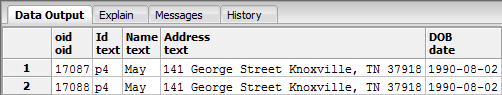
\includegraphics{F4.png}
\caption{Query on Person}
\label{fig:qonperson}
\end{figure}

\par
The tuples were not identical because they came from different tables and they had different OIDs. The same-value tuples did not violate the primary key constraint because table Person was empty. We can verify that by add ONLY keyword to the query and the query will return 0 result.
\begin{verbatim}
   SELECT oid, * FROM ONLY "Person";
\end{verbatim}

\par
The partition is not disjoint thus brings redundancy. We do not split the Person table in our design.

\subsubsection{References in PostgreSQL}
\label{sec:refinpgsql}
\par
In SQL 1999/2003 object extensions, we can use object references to access related objects in a way similar to object-oriented language, like Java. In PostgreSQL, we can define a column type as an existing table. For example, we can define ``owner'' column as Person type in table PerAccount. But it is actually store a Person tuple in the column, not a real reference. PostgreSQL does not provide reference types. Instead, PostgreSQL has a kind of object identifier types. For safety issues, PostgreSQL only uses OIDs as primary keys for various system tables. User-created tables are not recommended to use OIDs.
\par
Using OIDs in our tables does not simplify the query in our system. No function or call is provided to convert OID to object. If we want to get the object the OID represents, we have to do join query. Basically, it has nothing different from using our own foreign keys.
\par
When we create a foreign key that points to a supertable, we will encounter exception saying that foreign key does not exist. It is because the supertable is usually empty and PostgreSQL does not extract data from subtables when handle foreign key constraints. This type of behavior has been described in the document:
\par
\emph{All check constraints and not-null constraints on a parent table are automatically inherited by its children. Other types of constraints (unique, primary key, and foreign key constraints) are not inherited.}
\par
As a result, we need to handle the foreign key constraints which point to a supertable very carefully. We can create some triggers to ensure the data consistency. Or we can insert duplicate tuples to both supertable and subtable. In our design, we have a foreign key pointing to supertable Client from table Account. We keep a same copy of every tuple of subtables Organization and Person in supertable Client.
\par
In addition, PostgreSQL does not support array element foreign key referencing. In our original object-relational design, we have some array attributes in our classes. PostgreSQL can not define foreign key references on array. At first we want to use CHECK constraint, but those CHECK constraints in PostgreSQL does not support nested query.
\par
So we have to use triggers to ensure the references if we want to use arrays in our tables. Or we can use extra relationship tables and foreign keys in an old way. It is ARRAY + TRIGGERS vs TABLE + FOREIGN KEY. We choose the latter in our final design and we have three reasons:
\par
\begin{enumerate}
\item Using so many triggers is inefficient. For every many-to-many relationship, if we use arrays, we have to create triggers on every foreign key constraint. The triggers are for the action taken after update and delete. If we want to ensure participation constraints, we have to create triggers before insert. We do not want to write so many triggers. Using build-in foreign key constraints of PostgreSQL is fine with us.
\item Space efficiencies are asymptotically equal. Stroing the reference ids in array or table takes exactly the same space. Even if we compare the space taken by managing array structure or by managing new table, those two ways have same space complexities.
\item Class methods are global in PostgreSQL. We define some methods that return required tuples in our original design before. PostgreSQL stores all functions under schema, not table. That means if we move the array references out of table into a new relationship table, all functions in PostgreSQL have same accessibility.
\end{enumerate}
\par
So we decide to use extra relationship tables and foreign key references to store all many-to-many relationships. We also have some methods under the schema to provide us some object-oriented features to simplify our query.

\subsubsection{CCDB Database on PostgreSQL}
\par
PostgreSQL has some object-relational database features. But many of them are different from what we think about. In this section we cretae our CCDB system on PostgreSQL. Before we go into details, we create a new UML class diagram for CCDB under PostgreSQL, as shown in Figure \ref{fig:newumlccdb}.
\par
We remove the package Clients. Also, we omit all 0..* labels on association lines. Finally, all functions are grouped in a yellow box, which indicates the schema function library.

\begin{figure}[!htp]
\centering
\renewcommand{\umldrawcolor}{black}
\renewcommand{\umlfillcolor}{blue!10}
\begin{tikzpicture}
    \begin{class}[text width=4cm]{Account}{-2,0}
        \attribute{number : text}
        \attribute{balance : numeric}
        \attribute{limit : numeric}
        \attribute{owner : text}
    \end{class}

    \begin{class}[text width=4cm]{Client}{-2,-4}
        \attribute{id : text}
        \attribute{name : text}
        \attribute{address : text}
    \end{class}

    \begin{class}[text width=4cm]{Organization}{-6,-8}
        \inherit{Client}
    \end{class}
    \begin{class}[text width=4cm]{Person}{2,-8}
        \attribute{dob : date}
        \inherit{Client}
    \end{class}

    \begin{class}[text width=4cm]{Signs}{-2,-10}
        \attribute{pid : text}
        \attribute{oid : text}
    \end{class}

    \begin{class}[text width=4cm]{Authorizes}{5,0}
        \attribute{cid : text}
        \attribute{pid : text}
    \end{class}

    \draw [umlcd style] (Account) -- (Client) node[near start, right]{1..1};

    \draw [umlcd style] (Person.west |- 5, -8.5) -- (Organization.east |- -5, -8.5);

    \draw [umlcd style] (Account.east |- 5, -1) -- (2, -1);
    \draw [umlcd style] (2, -1) -- (2,-8);

    \draw [umlcd style dashed line] (-2, -8.5) -- (-2, -10);
    \draw [umlcd style dashed line] (2, -1) -- (Authorizes.west |- 5, -1);


    \node [draw, rectangle, align=left, fill=yellow!20] at (0, -15) {
 +getAuthUsers(Account) : Person[] \\
 +getOrgOwner(Account) : Organzation \\
 +getPerOwner(Account) : Person \\
 +getAccts(Organization) : Account[] \\
 +getAccts(Person) : Account[] \\
 +getSigners(Organization) : Person[] \\
 +getSignOrgs(Person) : Organization[] \\
 +getAuthAccts(Person) : Account[]};

\end{tikzpicture}
\caption{New UML diagram for CCDB}
\label{fig:newumlccdb}
\end{figure}


\paragraph{Using User-Defined Types in PostgreSQL}

\par
One of the important object-oriented features is user-defined types. PostgreSQL has UDTs but does not support the inheritance of UDTs. In our database, two UDTs are defined as accountType and clientType. The SQL commands are as follows:

\begin{verbatim}
CREATE TYPE public.accounttype AS
   ("number"  text,
    "balance" numeric,
    "limit"   numeric,
    "owner"   text);

CREATE TYPE public.clienttype AS
   ("id"     text,
    "name"    text,
    "address" text);
\end{verbatim}

\paragraph{Table Inheritance in PostgreSQL}
\par
PostgreSQL provides table inheritance. Based on the types and inheritance relationship, four tables are created as Account, Client, Organization and Person. We also create two relationship tables signs and authorizes. We include all primary key constraints and foreign key constraints as many as possible here.

\begin{verbatim}
CREATE TABLE public."Account"
OF accounttype
(
  "number" WITH OPTIONS  NOT NULL,
-- Inherited from type accounttype: balance,
-- Inherited from type accounttype: "limit",
  owner WITH OPTIONS  NOT NULL,
  CONSTRAINT account_pkey PRIMARY KEY (number),
  CONSTRAINT "Account_owner_fkey" FOREIGN KEY (owner)
      REFERENCES public."Client" (id) MATCH SIMPLE
      ON UPDATE CASCADE ON DELETE CASCADE
);

CREATE TABLE public."Client"
OF clienttype
(
  id WITH OPTIONS  NOT NULL,
-- Inherited from type clienttype: name,
-- Inherited from type clienttype: address,
  CONSTRAINT "Client_pkey" PRIMARY KEY (id)
);

CREATE TABLE public."Organization"
(
-- Inherited from table "Client":  id text NOT NULL,
-- Inherited from table "Client":  name text,
-- Inherited from table "Client":  address text,
  CONSTRAINT "Organization_pkey" PRIMARY KEY (id)
)
INHERITS (public."Client");

CREATE TABLE public."Person"
(
-- Inherited from table "Client":  id text NOT NULL,
-- Inherited from table "Client":  name text,
-- Inherited from table "Client":  address text,
  dob date,
  CONSTRAINT "Person_pkey" PRIMARY KEY (id)
)
INHERITS (public."Client");

CREATE TABLE public.signs
(
  pid text NOT NULL,
  oid text NOT NULL,
  CONSTRAINT signs_pkey PRIMARY KEY (pid, oid),
  CONSTRAINT signs_oid_fkey FOREIGN KEY (oid)
      REFERENCES public."Organization" (id) MATCH SIMPLE
      ON UPDATE CASCADE ON DELETE CASCADE,
  CONSTRAINT signs_pid_fkey FOREIGN KEY (pid)
      REFERENCES public."Person" (id) MATCH SIMPLE
      ON UPDATE CASCADE ON DELETE CASCADE
);

CREATE TABLE public.authorizes
(
  cid text NOT NULL,
  pid text NOT NULL,
  CONSTRAINT authorizes_pkey PRIMARY KEY (cid, pid),
  CONSTRAINT authorizes_cid_fkey FOREIGN KEY (cid)
      REFERENCES public."Account" ("number") MATCH SIMPLE
      ON UPDATE CASCADE ON DELETE CASCADE,
  CONSTRAINT authorizes_pid_fkey FOREIGN KEY (pid)
      REFERENCES public."Person" (id) MATCH SIMPLE
      ON UPDATE CASCADE ON DELETE CASCADE
);
\end{verbatim}

\paragraph{Triggers}
\par
We talked about we need triggers to ensure the constraints pointing to a supertable in section \ref{sec:refinpgsql}. Basically, we need to make supertable always has the tuples of its subtables. So we create triggers on Organization and Person. When the modify is done, do the same thing with supertable Client.

\begin{verbatim}
CREATE OR REPLACE FUNCTION public.tf_i_client()
  RETURNS trigger AS
$BODY$
  BEGIN
    INSERT INTO "Client" SELECT NEW.id, NEW.name, NEW.address;
    RETURN NEW;
  END;
$BODY$
  LANGUAGE plpgsql;

CREATE TRIGGER tf_i_organization
  AFTER INSERT
  ON public."Organization"
  FOR EACH ROW
  EXECUTE PROCEDURE public.tf_i_client();

 CREATE TRIGGER tf_i_person
  AFTER INSERT
  ON public."Person"
  FOR EACH ROW
  EXECUTE PROCEDURE public.tf_i_client();

CREATE OR REPLACE FUNCTION public.tf_u_client()
  RETURNS trigger AS
$BODY$
  BEGIN
    UPDATE ONLY "Client" SET id=NEW.id, name=NEW.name, address=NEW.address WHERE id=OLD.id;
    RETURN NEW;
  END;
$BODY$
  LANGUAGE plpgsql;

CREATE TRIGGER tf_u_organization
  AFTER UPDATE
  ON public."Organization"
  FOR EACH ROW
  EXECUTE PROCEDURE public.tf_u_client();

 CREATE TRIGGER tf_u_person
  AFTER UPDATE
  ON public."Person"
  FOR EACH ROW
  EXECUTE PROCEDURE public.tf_u_client();

CREATE OR REPLACE FUNCTION public.tf_d_client()
  RETURNS trigger AS
$BODY$
  BEGIN
    DELETE FROM "Client" WHERE id=OLD.id;
    RETURN NEW;
  END;
$BODY$
  LANGUAGE plpgsql;

CREATE TRIGGER tf_d_organization
  AFTER DELETE
  ON public."Organization"
  FOR EACH ROW
  EXECUTE PROCEDURE public.tf_d_client();

 CREATE TRIGGER tf_d_person
  AFTER DELETE
  ON public."Person"
  FOR EACH ROW
  EXECUTE PROCEDURE public.tf_d_client();
\end{verbatim}

\paragraph{Functions} PostgreSQL allows function overloading. We create several basic functions to satifsy our need. For the required query, we also create some helper functions. We will talk about that in section \ref{sec:qando}.
\label{sec:functions}
\begin{verbatim}
CREATE OR REPLACE FUNCTION public."getAuthUsers"("Account")
  RETURNS SETOF "Person" AS
' SELECT p.* FROM "Person" p, authorizes a WHERE $1.number = a.cid AND a.pid = p.id '
  LANGUAGE sql;

CREATE OR REPLACE FUNCTION public."getOrgOwner"("Account")
  RETURNS SETOF "Organization" AS
' SELECT * FROM "Organization" o WHERE o.id = $1.owner '
  LANGUAGE sql;

CREATE OR REPLACE FUNCTION public."getPerOwner"("Account")
  RETURNS SETOF "Person" AS
' SELECT * FROM "Person" p WHERE p.id = $1.owner '
  LANGUAGE sql;

CREATE OR REPLACE FUNCTION public."getAccts"("Organization")
  RETURNS SETOF "Account" AS
' SELECT * FROM "Account" a WHERE a.owner = $1.id '
  LANGUAGE sql;

CREATE OR REPLACE FUNCTION public."getAccts"("Person")
  RETURNS SETOF "Account" AS
' SELECT * FROM "Account" a WHERE a.owner = $1.id '
  LANGUAGE sql;

CREATE OR REPLACE FUNCTION public."getSigners"("Organization")
  RETURNS SETOF "Person" AS
' SELECT a.* FROM "Person" a, signs s WHERE $1.id = s.oid AND a.id = s.pid '
  LANGUAGE sql;

CREATE OR REPLACE FUNCTION public."getSignOrgs"("Person")
  RETURNS SETOF "Organization" AS
' SELECT o.* FROM "Organization" o, signs s WHERE $1.id = s.pid AND o.id = s.oid '
  LANGUAGE sql;

CREATE OR REPLACE FUNCTION public."getAuthAccts"("Person")
  RETURNS SETOF "Account" AS
' SELECT a.* FROM "Account" a, authorizes s WHERE $1.id = s.pid AND s.cid = a.number '
  LANGUAGE sql;
\end{verbatim}

\paragraph{Indexes} Query Optimizer can take advantage of indexes to produce better execution plans. We want to speed up our queries and improve the performance of our Web applications. Although we can create indexes for every column used in our queries, PostgreSQL would waste space and time to determine which indexes to use. Meanwhile, extra cost will be added into operations like inserts, updates and deletes since indexes need to be updated.
\par
To optimize the functions and the queries, we created 7 indexes in our database. We created an index on owner attribute of Account table since it is frequently used to join with Client, Organization and Person tables. We also considered to create an index on number attribute of Account table, but the effect was very limited and caused addition time on query 2. The id attributes of Organization and Person tables are also indexed. And finally, all attributes of authorizes and signs are indexed.

\begin{verbatim}
CREATE INDEX account_owner ON "Account" USING btree (owner);
CREATE INDEX organization_id ON "Organization" USING btree (id);
CREATE INDEX person_id ON "Person" USING btree (id);
CREATE INDEX signs_pid ON "signs" USING btree (pid);
CREATE INDEX signs_oid ON "signs" USING btree (oid);
CREATE INDEX authorizes_cid ON "authorizes" USING btree (cid);
CREATE INDEX authorizes_pid ON "authorizes" USING btree (pid);
\end{verbatim}

\section{Queries and Optimizations}
\label{sec:qando}
The queries are the same as Project 1. PostgreSQL has not support universal quantification, so we convert query 3 into double-negation form. As for query 4 and 5, we created recursive queries using common table expressions.
\par
To test the effect of optimization, we inserted 100,000 random tuples into Account, Organization and Person tables resepectively. Table authorizes and signs are also inserted 10,000 random tuples separately.

\subsection{Query 1}
Find all pairs of the form (user,signer), where user is an authorized user of an organization's credit card, signer is a person at that organization with signature authority, and the balance on the card is within \$1,000 of the credit limit. For each user/signer, show Id and Name.
\par
In this query, we treat ``authorized user'' as non-owner-and-signer authorized user to fit the test data sample output.

\paragraph{Supporting functions} We already have all the supporting functions defined. What we need are getAuthUsers(Account), getOOwner(Account) and getSigners(Organization) in section \ref{sec:functions}.

\paragraph{Query SQL statement} Using functions we talked above, we can build our query statement succinctly.
\begin{verbatim}
SELECT au.id, au.name, s.id, s.name
FROM "Account" oa, "getAuthUsers"(oa) au, "getOrgOwner"(oa) oo, "getSigners"(oo) s
WHERE oa.balance - oa.limit <= 1000 AND oa.balance - oa.limit >= -1000;
\end{verbatim}

\paragraph{Optimization} Table \ref{tab:q1} shows the join fields of Query 1.

\begin{table}[!htbp]
\centering
\label{tab:q1}
\caption{Join table of Query 1}
\begin{tabular}{|l||r|c|l|c|}
\hline
{\itshape Function} & \multicolumn{4}{c|}{\itshape Join} \\
\hline
\multirow{2}{*}{getAuthUsers} & 1 & Account.number & - & authorizes.cid \\
\cline{2-5}
& 2 & authorizeds.pid & - & Person.id \\
\hline
getOrgOwner & 3 & Account.owner & - & Organization.id \\
\hline
\multirow{2}{*}{getSigners} & 4 & Organization.id & - & signs.oid \\
\cline{2-5}
& 5 & signs.pid & - & Person.id \\
\hline
\end{tabular}
\end{table}

\par
Although there are 5 joins in Query 1, the optimization effect of indexes is not obvious. This may be we haven't insert enough data into tables. Or the where clause of Query 1 reduces many tuples at the beginning. The query runtimes before and after optimization are all 1.3 seconds.

\subsection{Query 2}
Find all users (Id, Name) who own four or more cards and are authorized non-owner users for three or more other cards.

\paragraph{Supporting functions} We defined two supporting functions to this query: getAcctNum(Person) and getAuthAcctNum(Person).
\begin{verbatim}
CREATE OR REPLACE FUNCTION public."getAcctsNum"("Person")
  RETURNS bigint AS
' SELECT count(*) FROM "getAccts"($1)'
  LANGUAGE sql;

CREATE OR REPLACE FUNCTION public."getAuthAcctsNum"("Person")
  RETURNS bigint AS
' SELECT count(*) FROM "getAuthAccts"($1) '
  LANGUAGE sql;
\end{verbatim}

\paragraph{Query SQL statement}
\begin{verbatim}
SELECT p.id, p.name
FROM "Person" p
WHERE "getAcctsNum"(p)>=4 AND "getAuthAcctsNum"(p)>=3;
\end{verbatim}

\paragraph{Optimization} Table \ref{tab:q2} shows the join fields of Query 2.

\begin{table}[!htbp]
\centering
\label{tab:q2}
\caption{Join table of Query 2}
\begin{tabular}{|l||r|c|l|c|}
\hline
{\itshape Function} & \multicolumn{4}{c|}{\itshape Join} \\
\hline
getAcctsNum & 1 & Person.id & - & Account.owner \\
\hline
\multirow{2}{*}{getAuthAcctsNum} & 2 & Person.id & - & authorizes.pid \\
\cline{2-5}
& 3 & authorizes.cid & - & Account.number \\
\hline
\end{tabular}
\end{table}

\par
The optimization effect in Query 2 is very significant. The runtime before optimization is 18 minutes 47 seconds while 5.6 seconds is the runtime after optimization.

\subsection{Query 3}
Find the credit cards (acct. numbers) all of whose signers (i.e., people with signature authority of the organizations that own those cards) also own personal credit cards with credit limits at least \$25,000.

\paragraph{Supporting functions} We defined one supporting function getMaxLimit(Person) to this query.
\begin{verbatim}
CREATE OR REPLACE FUNCTION public."getMaxLimit"("Person")
  RETURNS numeric AS
' SELECT max(a.limit) FROM "getAccts"($1) a '
  LANGUAGE sql;
\end{verbatim}

\paragraph{Indexes}
\begin{verbatim}
CREATE INDEX organization_id_index
  ON "Organization"
  USING btree
  (id COLLATE pg_catalog."default");

CREATE INDEX person_id_key
  ON "Person"
  USING btree
  (id COLLATE pg_catalog."default");
\end{verbatim}

\paragraph{Query SQL statement} Since PostgreSQL does not support universal quantification, we have to use double-negation to create equivalent query. We convert ``for all ... at least'' to ``not exist ... less than''.
\begin{verbatim}
SELECT DISTINCT a.number
FROM "Account" a, "getOrgOwner"(a) oo, "getSigners"(oo) s
WHERE NOT "getMaxLimit"(s) < 25000;
\end{verbatim}

\paragraph{Optimization} Table \ref{tab:q3} shows the join fields of Query 3.

\begin{table}[!htbp]
\centering
\label{tab:q3}
\caption{Join table of Query 3}
\begin{tabular}{|l||r|c|l|c|}
\hline
{\itshape Function} & \multicolumn{4}{c|}{\itshape Join} \\
\hline
getOrgOwner & 1 & Account.owner & - & Organization.id \\
\hline
\multirow{2}{*}{getSigners} & 2 & Organization.id & - & signs.oid \\
\cline{2-5}
& 3 & signs.pid & - & Person.id \\
\hline
getMaxLimit & 4 & Account.owner & - & Person.id \\
\hline
\end{tabular}
\end{table}

\par
The optimization effect in Query 3 is not obvious. The runtime before optimization is 1012 milliseconds while 845 milliseconds is the runtime after optimization.

\subsection{Query 4}
Find all pairs (U,C) where U is an indirect user of the credit card C. (For each user, show Id and Name. For credit cards, show the account number.)

\paragraph{Supporting functions} We need to define a new function that returns proper authorized users. Basically it is getAuthUsers function plus getSigners if the card owner is an organization.
\begin{verbatim}
CREATE OR REPLACE FUNCTION public."getNonOwnerAuthUsers"("Account")
  RETURNS SETOF "Person" AS
$BODY$
  SELECT p.*
  FROM "Person" p, authorizes a
  WHERE $1.number = a.cid AND a.pid = p.id
  UNION
  -- union signer if owner is an organization
  SELECT p.*
  FROM "Person" p, signs s
  WHERE $1.owner = s.oid AND s.pid = p.id
$BODY$
  LANGUAGE sql;
\end{verbatim}

\paragraph{Query SQL statement} WITH statement (CTE) is used in this query to do recursive query.
\begin{verbatim}
WITH RECURSIVE indirect_user(id, name, number) AS (
    SELECT aa.id, aa.name, a.number
    FROM "Account" a, "getNonOwnerAuthUsers"(a) aa
  UNION
    SELECT aa.id, aa.name, iu.number
    FROM indirect_user iu, "Account" a, "getNonOwnerAuthUsers"(a) aa
    WHERE iu.id = a.owner
)
SELECT *
FROM indirect_user;
\end{verbatim}

\paragraph{Optimization} Table \ref{tab:q4} shows the join fields of Query 4.

\begin{table}[!htbp]
\centering
\label{tab:q4}
\caption{Join table of Query 4}
\begin{tabular}{|l||r|c|l|c|}
\hline
{\itshape Function} & \multicolumn{4}{c|}{\itshape Join} \\
\hline
\multirow{4}{*}{getNonOwnerAuthUsers} & 1 & Account.number & - & authorizes.cid \\
\cline{2-5}
& 2 & authorizes.pid & - & Person.id \\
\cline{2-5}
& 3 & Account.owner & - & signs.oid \\
\cline{2-5}
& 4 & signs.pid & - & Person.id \\
\hline
indirectUser & 5 & indirectUser.id & - & Account.owner \\
\hline
\end{tabular}
\end{table}

\par
The optimization effect in Query 4 is obvious. The runtime before optimization is 8 minutes and 4 seconds while 10.4 seconds is the runtime after optimization.

\subsection{Query 5}
Find the total of all balances for the credit cards that have Joe as one of the indirect users.

\paragraph{Supporting functions} Same as Query 4.

\paragraph{Query SQL statement} WITH statement (CTE) is used in this query to do recursive query.
\begin{verbatim}
WITH RECURSIVE indirect_user(id, name, number) AS (
    SELECT aa.id, aa.name, a.number
    FROM "Account" a, "getNonOwnerAuthUsers"(a) aa
  UNION
    SELECT aa.id, aa.name, iu.number
    FROM indirect_user iu, "Account" a, "getNonOwnerAuthUsers"(a) aa
    WHERE iu.id = a.owner
)
SELECT sum(a.balance)
FROM indirect_user iu, "Account" a
WHERE iu.name = 'Joe' AND iu.number = a.number;
\end{verbatim}

\paragraph{Optimization} Table \ref{tab:q5} shows the join fields of Query 5.

\begin{table}[!htbp]
\centering
\label{tab:q5}
\caption{Join table of Query 5}
\begin{tabular}{|l||r|c|l|c|}
\hline
{\itshape Function} & \multicolumn{4}{c|}{\itshape Join} \\
\hline
\multirow{4}{*}{getNonOwnerAuthUsers} & 1 & Account.number & - & authorizes.cid \\
\cline{2-5}
& 2 & authorizes.pid & - & Person.id \\
\cline{2-5}
& 3 & Account.owner & - & signs.oid \\
\cline{2-5}
& 4 & signs.pid & - & Person.id \\
\hline
indirectUser & 5 & indirectUser.id & - & Account.owner \\
\hline
SELECT & 6 & indirectUser.number & - & Account.number \\
\hline
\end{tabular}
\end{table}

\par
The optimization effect in Query 5 is same as Query 4. The runtime before optimization is 8 minutes and 21 seconds while 10.5 seconds is the runtime after optimization.

\section{CCDB System Interface}
The interface to our CCDB system is realized with the front end JSP webpage and the back end servlet. A webpage provides an interface where users are able to invoke one of the five queries described in section \ref{sec:qando}. The servlet is responsible for interacting with the database and returning the query results to the browser.
\subsection{Front End JSP}
A JSP is a webpage combining the traditional HTML and Java code. In our webpage, five links are available for each query; clicking a link is viewed as sending a request to the servlet. Furthermore, calling the servlet is achieved using JavaScript.
\begin{verbatim}
<ul class="submenu">
    <li><a href="#" onclick="javascript: query(1);">Query 1</a></li>
    <li><a href="#" onclick="javascript: query(2);">Query 2</a></li>
    <li><a href="#" onclick="javascript: query(3);">Query 3</a></li>
    <li><a href="#" onclick="javascript: query(4);">Query 4</a></li>
    <li><a href="#" onclick="javascript: query(5);">Query 5</a></li>
</ul>

<script language="JavaScript">
    function query(id) {
        resulttable.innerHTML = "<iframe src=\"QueryProcessingServlet?Query=" + id + "\"
                                scrolling=\"no\"></iframe>";
    }
</script>
\end{verbatim}

\subsection{Back End Servlet}
The servlet, which is indeed a Java class named QueryProcessingServlet, generates dynamic HTML content showing the query results. It receives the request from JSP, processes such request, and constructs a response sent back to the browser. Detailed servlet's tasks are described as follows.

\subsubsection{Establish a Connection to the CCDB}
With the use of JDBC driver, the servlet initiates a connection to the CCDB system.
\begin{verbatim}
// Load JDBC driver
Class.forName("JDBC.driver");

// Create a connection
// DatabaseURL: our CCDB url (e.g. "jdbc:postgresql://127.0.0.1:5432/ccdb")
Connection conn = DriverManager.getConnection( DatabaseURL, UserName, Password);
\end{verbatim}

\subsubsection{Create a SQL Statement and Obtain the Results}
The servlet creates a SQL statement for sending a SQL query to the database and obtaining the produced results.
\begin{verbatim}
Statement stmt = conn.createStatement(ResultSet.TYPE_SCROLL_SENSITIVE, ResultSet.CONCUR_UPDATABLE);

// sql is a String object containing one of our five SQL queries.
ResultSet rs = stmt.executeQuery(sql);
\end{verbatim}

\subsubsection{Return Query Results to the Browser}
The servlet creates a PrintWriter object to compose a text-output stream. The stream integrates the query results into the HTML content so that the browser is able to render it.
\begin{verbatim}
HttpServletResponse response;
PrintWriter out = response.getWriter();

out.println( "<table>" );

// Print the attributes
out.println( "<thead> <TR>" );
for( int i = 1; i <= columnCnt; ++i )
{
    String label = rs.getMetaData().getColumnLabel( i );
    out.println( "<TD><b>"+ label +"</b></TD>" );
}
out.println( "</thead> </TR>" );

// Print the values
while (rs.next())
{
    out.println( "<TR align='left'>" );
    for( int i = 1; i <= columnCnt; ++i )
    {
        out.println( "<TD>"+ rs.getString(i) +"</TD>" );
    }
    out.println( "</TR>" );
}

out.println( "</table>" );
\end{verbatim}

\section{Results}
A user first opens a browser and types the URL (\url{http://localhost:8080/ccdb_oo/index.jsp}) to connect to the server. Then, a webpage allowing the user to select a SQL query shows up. Once a query is invoked, a table consisting of query results will be displayed. Figure \ref{fig:resultccdb} shows a sample result in which the user invokes the first query.

\begin{figure}[!htp]
\centering
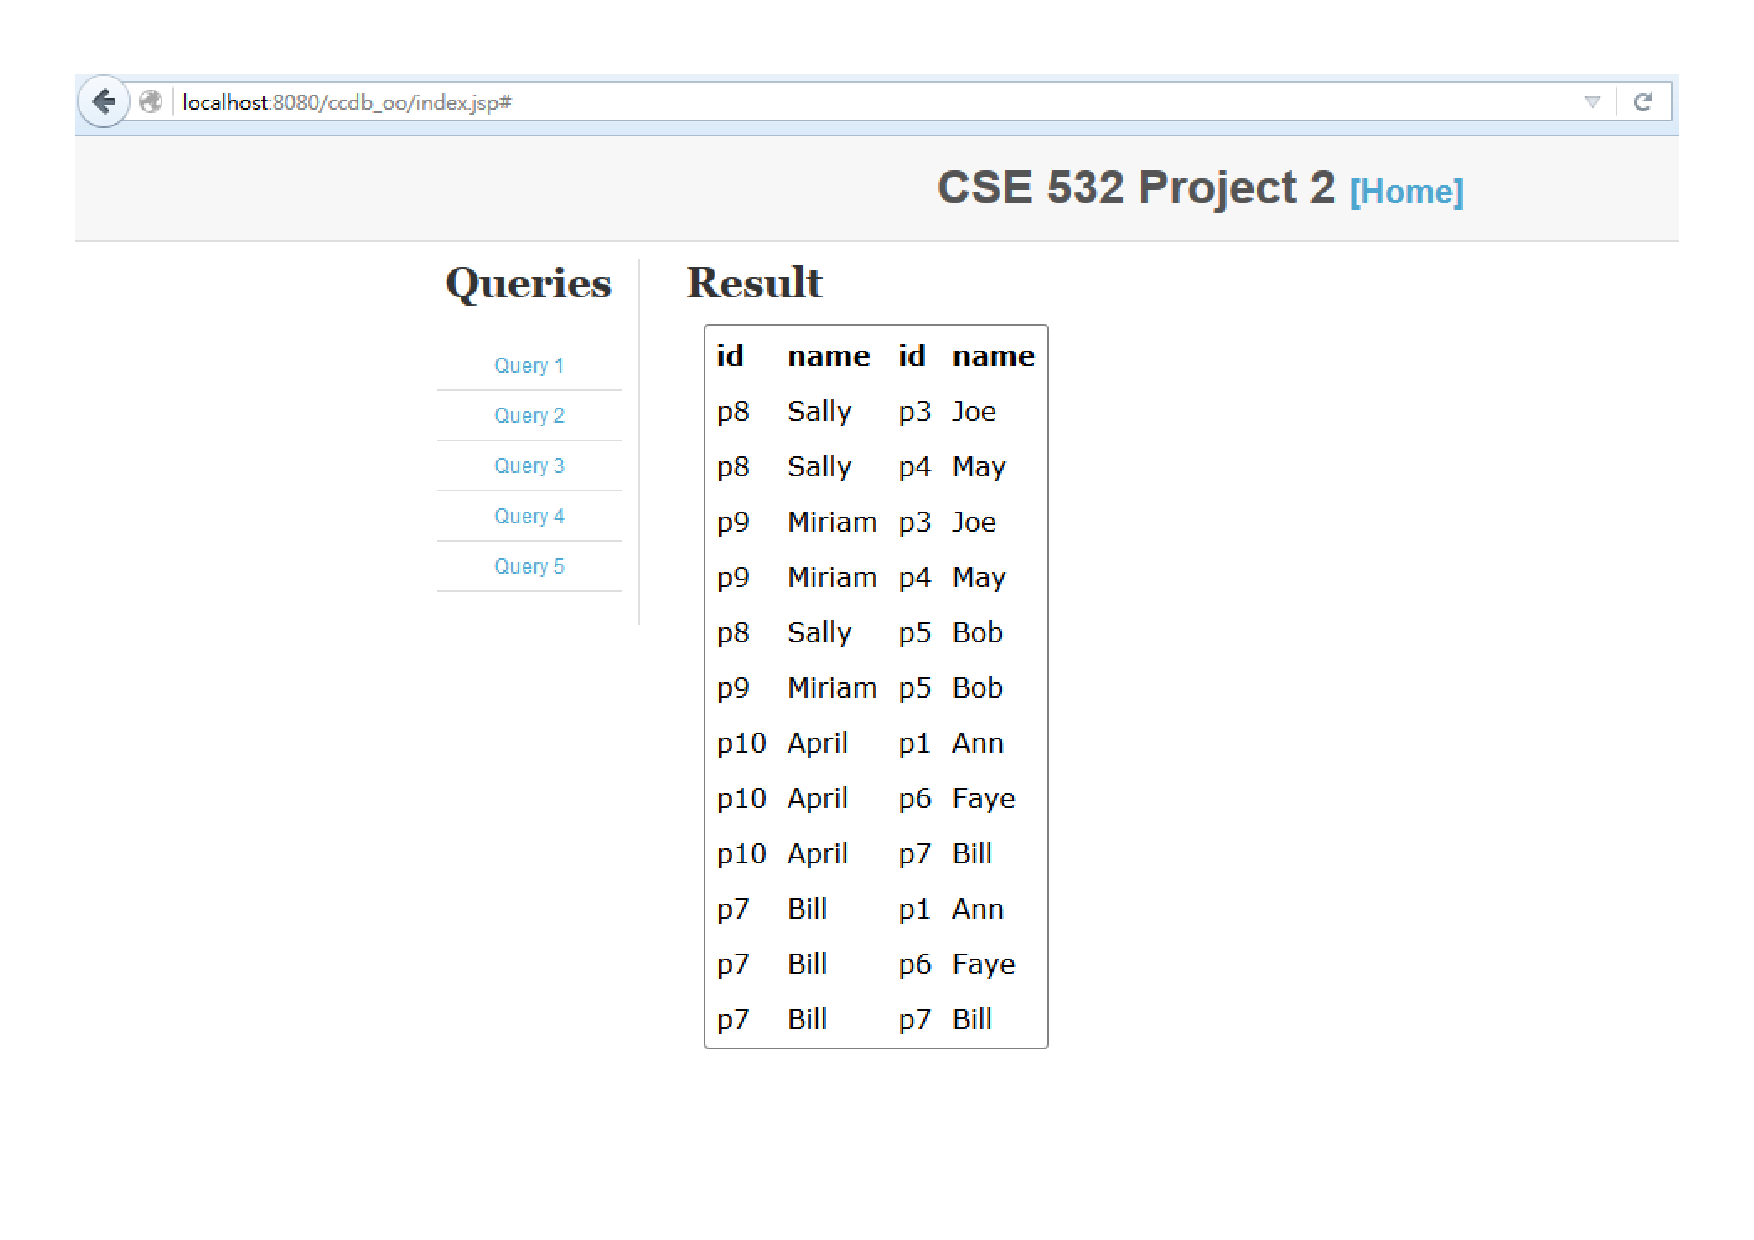
\includegraphics[width=7in]{result.pdf}
\caption{Result of the first query}
\label{fig:resultccdb}
\end{figure}

\end{document}
